\documentclass[a4paper,12pt]{article}
\usepackage{amsmath}  % For equations
\usepackage{amsfonts} % For mathematical symbols
\usepackage{graphicx} % For figures
\usepackage{hyperref} % For links
\usepackage{appendix} % For appendices
\usepackage [round,authoryear] {natbib}

\DeclareMathOperator*{\argmax}{argmax}
\DeclareMathOperator*{\argmin}{argmin}

\usepackage{amsthm}
\usepackage{xcolor}

\theoremstyle{definition}
\newtheorem{exinn}{Example}
\newtheorem{theorem}{Theorem}
\newtheorem{definition}{Definition}

\newenvironment{example}
{\clubpenalty=10000
	\begin{exinn}%
		\mbox{}%
		{\color{black}\leaders\hrule height .8ex depth \dimexpr-.8ex+0.8pt\relax\hfill}%
		\mbox{}\linebreak\ignorespaces}
	{\par\kern2ex\hrule\end{exinn}}


\title{Sequential Decision-Making for Inventory Control using Bayesian Decision Theory}
\author{Jonas Petersen \\ Ander Runge Walther }
\date{\today}

\begin{document}
	\maketitle
	
	\begin{abstract}
		Inventory control is a core aspect of supply chain management, balancing customer demand fulfillment against the costs of holding and ordering inventory. This paper addresses inventory management through the lens of Bayesian decision theory, enabling probabilistic decision-making under uncertainty. By establishing a framework for sequential decision-making over an infinite time horizon, an optimal solution tailored to a specific asymmetric cost function is derived, offering insights for practical implementations in inventory management.
	\end{abstract}
	
	\section{Introduction}
	Inventory management is a critical component of supply chain management that involves overseeing the ordering, storage, and use of a company's inventory, including raw materials, components, and finished goods. Effective inventory control ensures that a company has adequate stock to meet demand while minimizing costs associated with holding inventory. In practice, this often requires a balance between minimizing stockouts, which disrupt service levels, and limiting overstocking, which incurs unnecessary holding costs.
	
	The coordination of inventory and transportation decisions has gained significant attention over recent decades, driven by the need for specific practices like vendor-managed inventory (VMI), third-party logistics (3PL), and time-definite delivery (TDD) (see, e.g., \citep{CetinkayaLee2000, Alumur2012, Gurler2014}). These programs aim to optimize the balance between inventory holding costs and transportation costs. Traditional inventory models often assume immediate delivery to meet demand, yet this can be inefficient due to the fixed costs of transportation, prompting companies to adopt shipment consolidation policies that merge smaller demands into larger, less frequent shipments \citep{CetinkayaBookbinder2003, HigginsonBookbinder1994}.
	
	Three commonly implemented shipment consolidation policies—quantity-based, time-based, and hybrid—are particularly useful in improving cost efficiency by regulating shipment size or timing. Each policy type has distinct impacts on performance metrics, such as delay penalties, average inventory, and annual costs, guiding companies toward designing more efficient inventory-transportation systems \citep{Cetinkaya2005, Wei2020, Cetinkaya2006}.
	
	While these approaches provide valuable frameworks, they do not explicitly account for the uncertainties inherent in demand fluctuations or the associated asymmetric costs of overstocking and understocking. In settings where inventory decisions must be made sequentially, uncertainty can be more effectively managed through Bayesian decision theory, which offers a probabilistic approach to decision-making under uncertainty. This framework allows for more refined, sequential adjustments to inventory based on demand forecasting, which dynamically incorporates new data over time.
	
	In this study, Bayesian decision theory is utilized to address a sequential inventory control problem. Specifically, an optimal decision-making framework is derived based on a discounted asymmetric cost function, considering the impact of decisions made infinitely far into the future. Our model involves a decision-maker (henceforth referred to as the Robot) who manages stock levels over time in an interactive environment shaped by a random demand process. Through this setup, a mathematically rigorous and computationally feasible solution for optimal inventory decisions that account for uncertainty and asymmetric costs is derived.
	
	\section{Sequential Decision-Making Framework}
	To formalize the sequential decision-making problem, consider a stock management scenario in which the Robot makes decisions at each time step, interacting with an entity termed Nature, which represents environmental randomness~\citep{lavalle2006}. At each iteration $t$, the Robot decides on an action from its action space $\Omega_U$, while Nature removes a certain number of units from stock, denoted $s_t \in \Omega_S$. The goal is to manage the stock optimally, balancing the costs of overstocking ($N > 0$) and understocking ($N < 0$), given that each action taken has a probabilistic effect on the Robot’s objectives.
	
	The Robot’s decisions are based on historical data $D$, which contains past stock removals and other relevant demand features. Given an initial stock $N_0$, the stock level at time $t$ evolves according to
	\begin{equation}
		\begin{split}
			N_t &\equiv N_0 + \sum_{t'=1}^{t} (U_{t'-L} - s_{t'})\\
			& = N_0+\upsilon_t-\zeta_t
		\end{split},
	\end{equation}
	where $U_{t'-L}$ represents the decision made at an earlier time due to a potential lag $L$ and $\zeta_t\equiv \sum_{t'=1}^ts_{t'}$ and $\upsilon_t\equiv \sum_{t'=1}^tU_{t'-L}$. To support probabilistic decision-making, the Robot uses a forecast based on $D$ in the form
	\begin{equation}
		p(s_1, s_2, \dots | D, I),
	\end{equation}
	where $I$ denotes any additional background information~\citep{Sivia2006}. This probabilistic forecast, combined with the Robot's asymmetric cost function, guides the sequence of decisions over time.
	
	\section{Formulation of the Cost Function and Optimal Decision Rule}
	The Robot’s objective is to formulate a sequence of decision rules, called a policy, $\xi = \{U_0(D), U_1(D), \dots\}$, where each $U_j(D) = u_j$ minimizes the expected cost
	\begin{equation}
		\xi^* = \arg \min_{\xi} \mathbb{E}[C | D, I],
	\end{equation}
	where the cost $C$ is assumed to be discounted viz
	\begin{equation}
		C = \sum_{t=1}^{\infty} \gamma_{\text{disc}}^{t} \left( h_t 1_{N_t> 0} + c_t (1_{N_t> 0}-1) \right)N_t,
		\label{eq:cost}
	\end{equation}
	where $\gamma_{\text{disc}} \in [0,1]$ is a discount factor, and $h$ and $c$ represent storage (holding) and understocking costs, respectively. The optimal decisions satisfy the first-order condition
	\begin{equation}
		\frac{d}{dU_m} \mathbb{E}[C | D, I] \Big|_{U_m = U_m^*} \overset{!}{=} 0 \quad \forall m,
		\label{eq:min_exp_cost}
	\end{equation}
	which leads to the optimal decision criterion (see Appendix~\ref{app:deriva} for a detailed derivation).
	
	\begin{theorem}[Optimal Policy Rule for Inventory Control]
		Given the sequential decision-making framework and the asymmetric cost function in equation \eqref{eq:cost}, the optimal policy for the Robot at each time step $t$ is defined by
		\begin{equation}
			p(N_t^* > 0 | D, I) = \frac{c_t}{c_t + h_t},
		\end{equation}
		where
		\begin{equation}
			N_t^* = N_0 +\upsilon_t^*-\zeta_t.
		\end{equation}
	\end{theorem}
	
	This criterion implies that the optimal decisions correspond to the quantile threshold
	\begin{equation}
		\upsilon_t^* = Q_{\frac{c_t}{c_t+h_t}}\zeta_t-N_0,
		\label{eq:opt}
	\end{equation}
	where $Q_q(X)$ denotes the $q$-quantile of the random variable $X$. This result provides an actionable rule for the Robot’s decision-making based on the balance of costs associated with stock levels.
	
	\section{Cost Efficiency Ratio}
	In order to illustrate implementation and the order of magnitude effect from using the optimal decision rule, consider the ratio
	\begin{equation}
		\frac{\mathbb{E}[C^*|D,I]}{\mathbb{E}[C'|D,I]},
	\end{equation}
	where $C^*$ is the cost function with the optimal policy and $C'$ is the baseline policy defined viz
	
	\begin{definition}[baseline policy]
		The baseline policy consists of ordering the expected value $\mathbb{E}[s_t|D,I]$ if $N_t<\mathbb{E}[s_t|D,I]$.
	\end{definition}
	
	The baseline policy represents an (R,Q) policy with the reorder point $N_t=0$ and batch quantity $\mathbb{E}[s_t|D,I]$. This policy is a simple approach to keeping the stock as close as possible to the reorder point while favoring a positive stock. Assuming $p(\zeta_t|D,I)$ follow a Poisson distribution, the CER can be approximated (see appendix \ref{app:cer})
	\begin{equation}
		\frac{\mathbb{E}[C^*|D,I] }{\mathbb{E}[C'|D,I]}\sim \frac{1}{1+\frac{2h}{c}}
	\end{equation}
	
	
	
	\begin{figure}[h!]
		\centering
		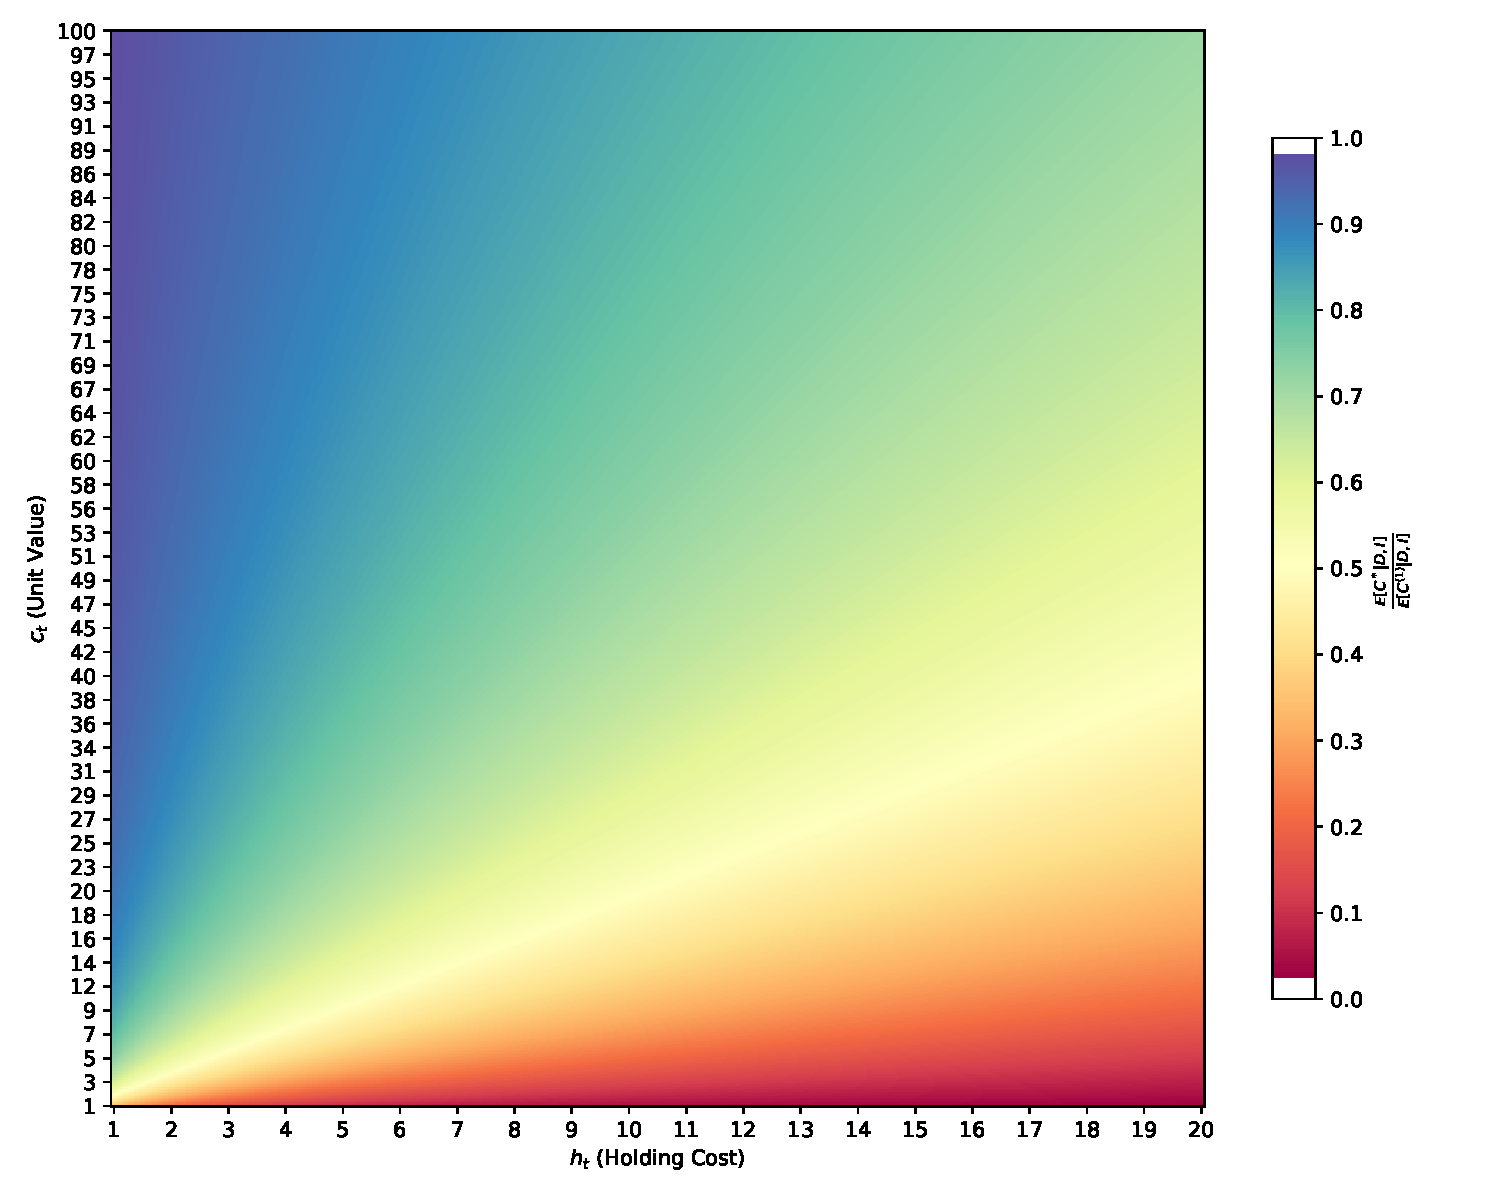
\includegraphics[width=\textwidth]{figures/analytical_heatmap.pdf}
		\caption{Heatmap of Cost Improvements}
		\label{fig:heatmap_analytical}
	\end{figure}
	
	
	
	For the numerical example, consider $k_t=k,c_t=c$ for a range of constant (over time) values $k,c$.
	
	\begin{figure}[h!]
		\centering
		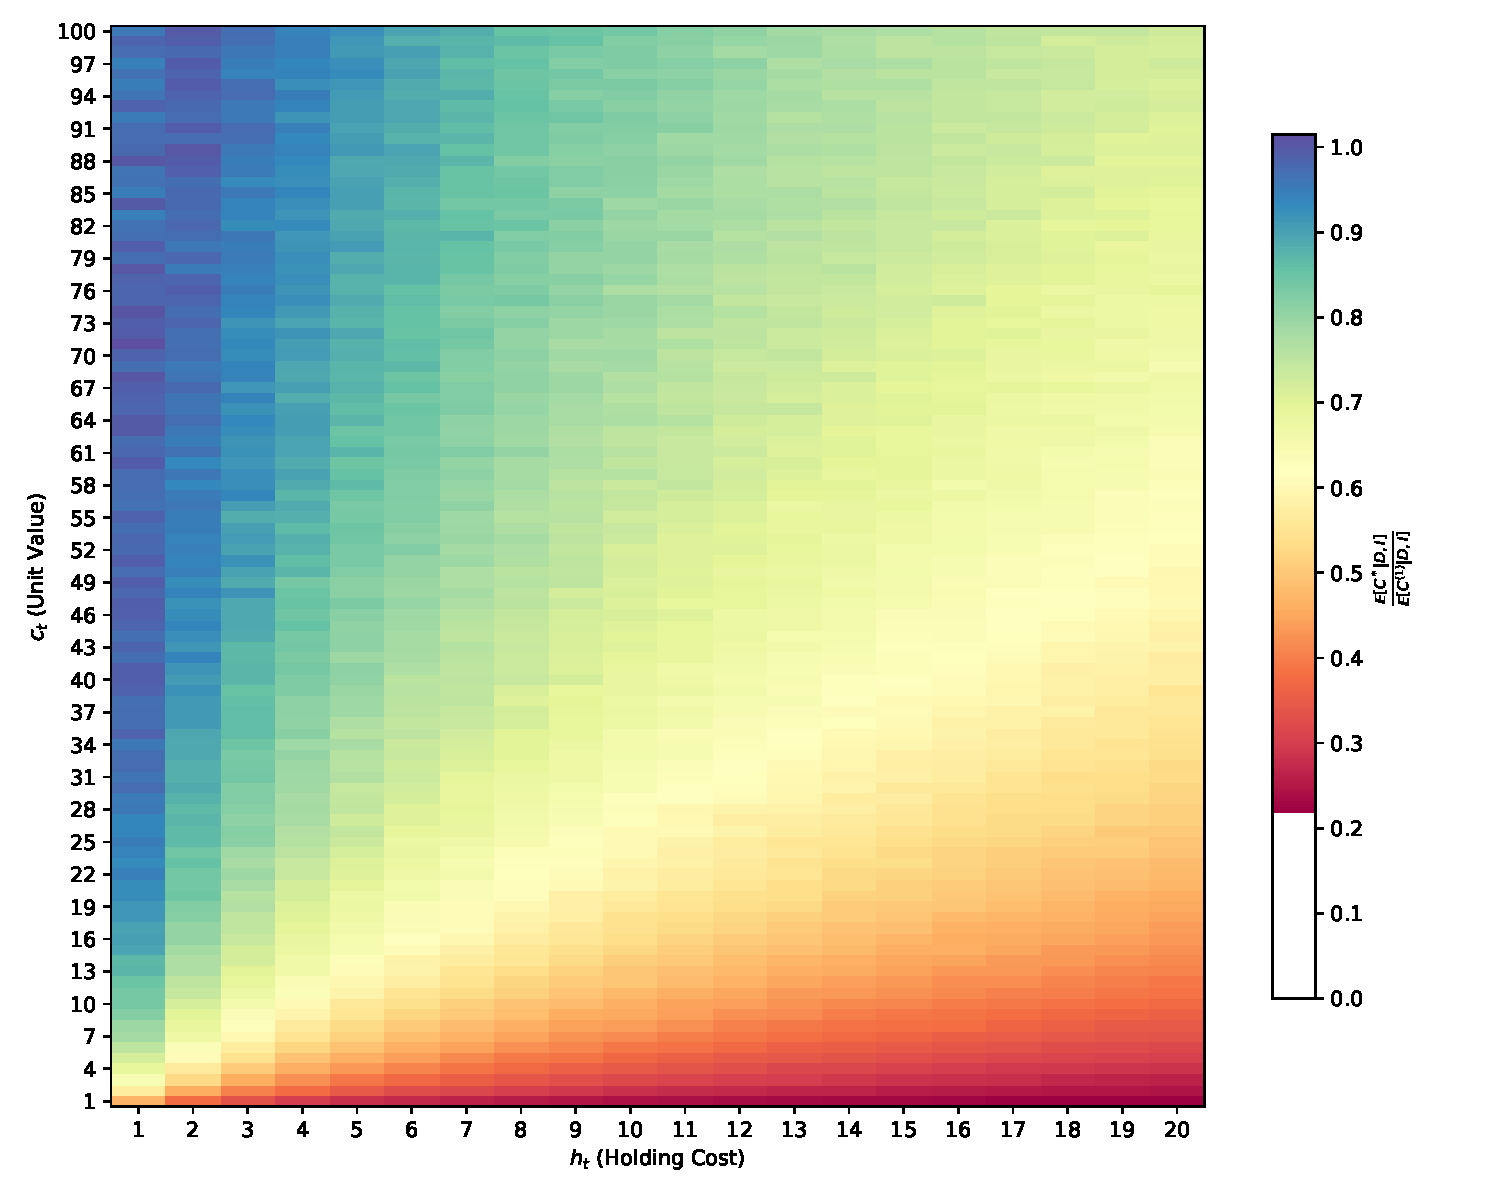
\includegraphics[width=\textwidth]{figures/numerical_heatmap.pdf}
		\caption{Heatmap of Cost Improvements}
		\label{fig:heatmap}
	\end{figure}
	
	From the figure it is clear that
	
	\begin{equation}
		\frac{\mathbb{E}[C^*|D,I]}{\mathbb{E}[C'|D,I]}\bigg|_{\frac{h_t}{c_t} = \text{const}, h_t\neq 0}\sim \text{const},
	\end{equation}

	this means for any $h_t\neq 0$, $\frac{\mathbb{E}[C^*|D,I]}{\mathbb{E}[C'|D,I]}$ can be analyzed as a function of $c_t$ in a general scope. {\color{red} Does it mean the fraction is a function of $h/c$ ?}
	
	\begin{figure}[h!]
		\centering
		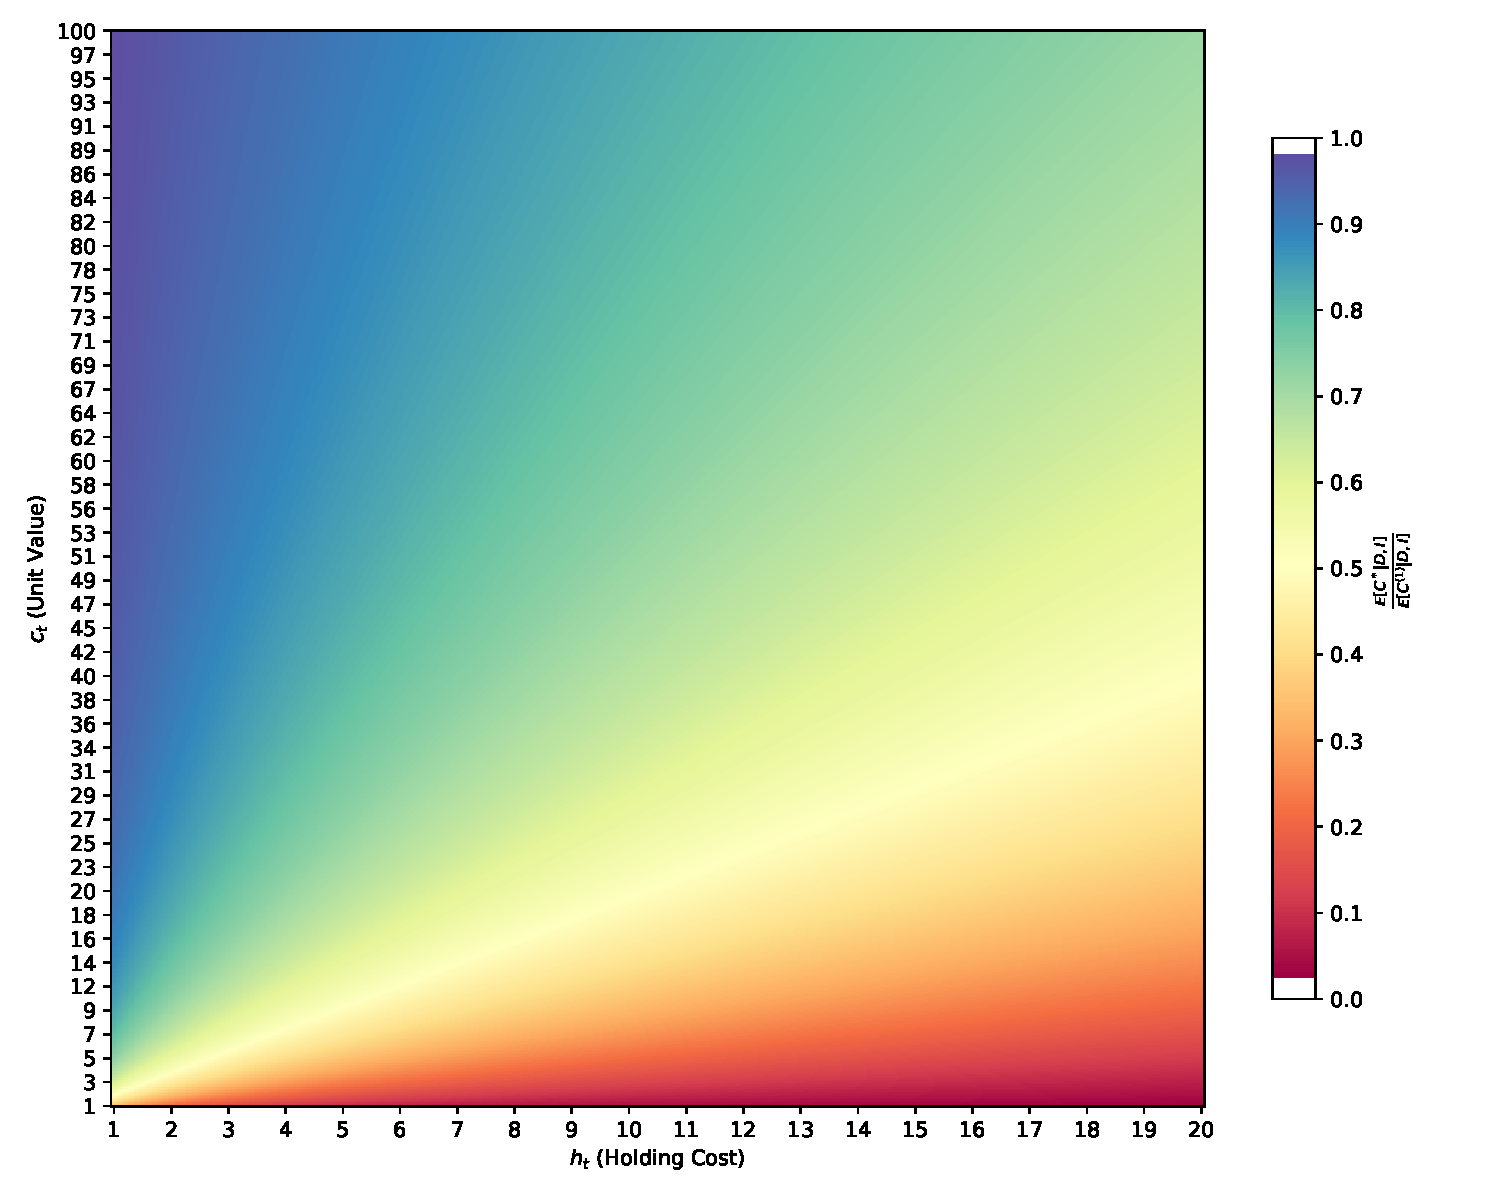
\includegraphics[width=\textwidth]{figures/analytical_heatmap.pdf}
		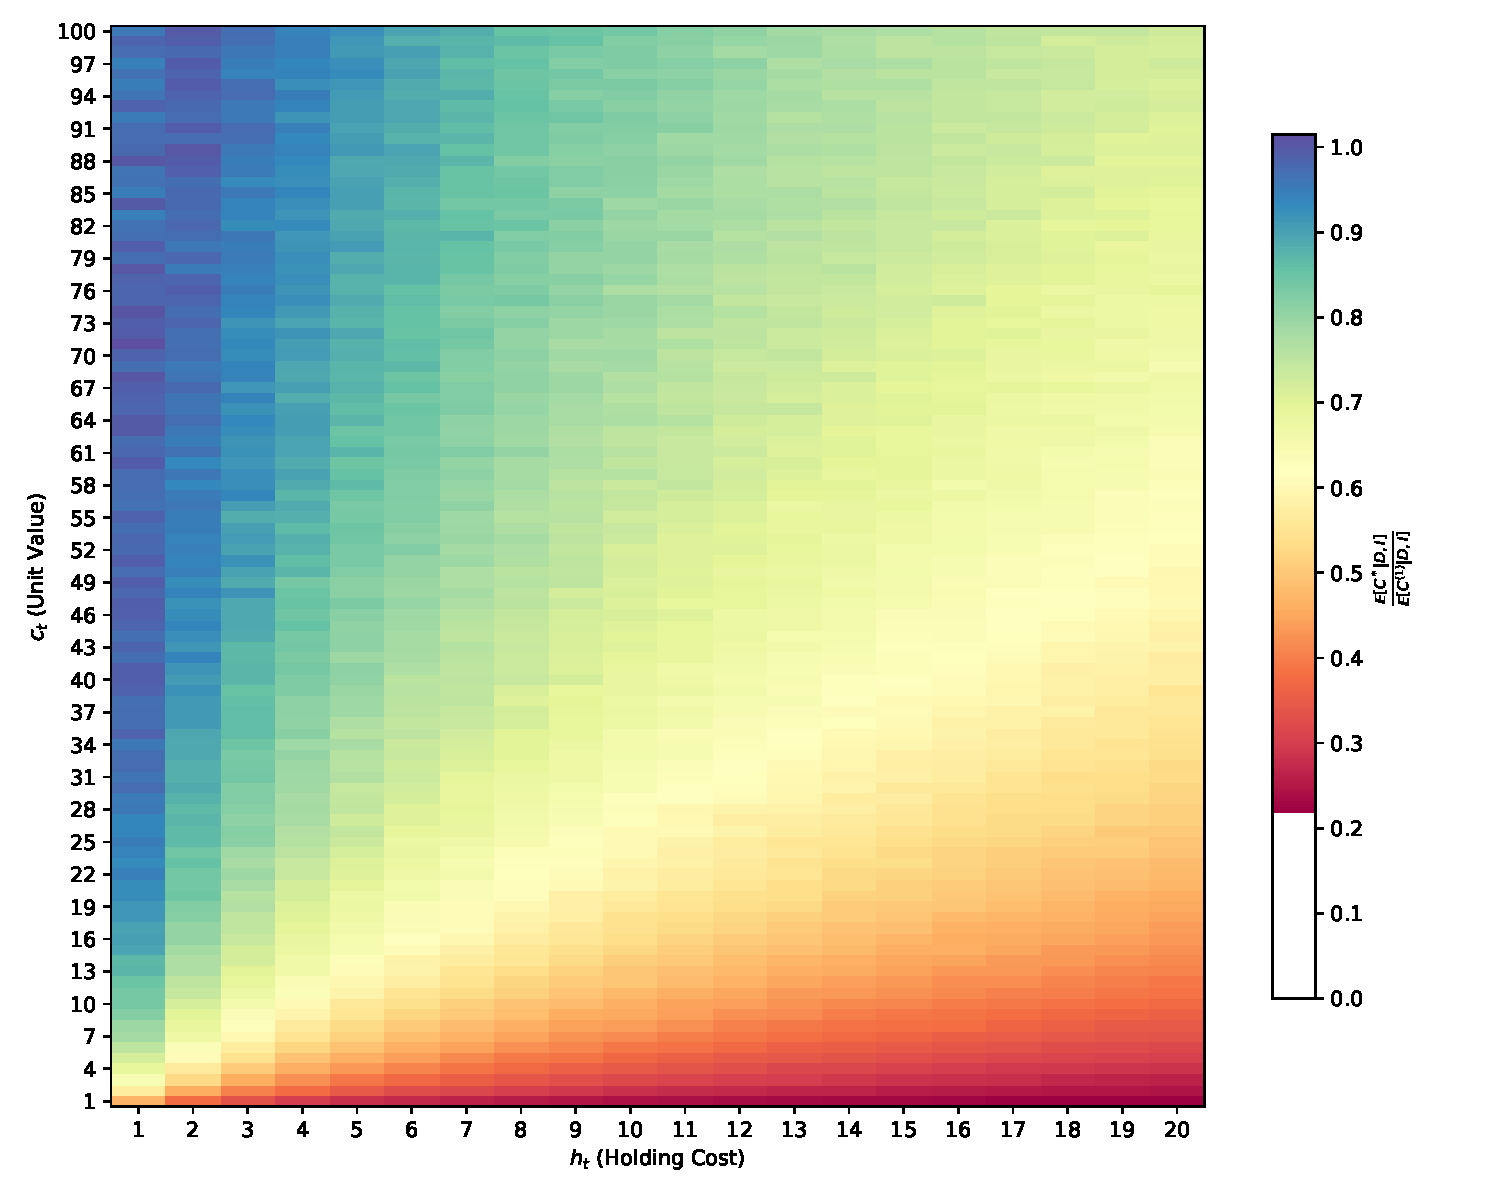
\includegraphics[width=\textwidth]{figures/numerical_heatmap.pdf}
		\caption{Heatmap of Cost Improvements}
	\end{figure}
	
	=================
	

	
	\section{Conclusion}
	The derived decision rule offers a structured approach to managing inventory in a stochastic environment using Bayesian decision theory. The probabilistic framework accounts for demand uncertainty, guiding optimal actions based on expected costs. This work contributes to the field of inventory management by presenting an analytically derived solution, supporting practical applications in real-world inventory systems.
	
	\begin{enumerate}
		\item A few words on the intuitive interpretation of the cost function? The number of units overstocked multiplied with the cost of overstocking per unit. The number of units understocked multiplied with the value of each unit. The latter represents the lost value.
		\item Mention the benefit of the analytical solution; the computation speed relative to a numerical optimization is highly beneficial at scale.
		\item Compress the recursive relation to $m$-notation. 
		\item The baseline policy is an (R,Q) policy with $R =0$ and $Q = \mathbb{E}[s_t|D,I]$.
		\item Is our result in any of the inventory control books?
		\item will the relationship between baseline and optimal policy depend on forecasting method? I would say yes. How do we handle this?
		
		\item if there is around the same cost for over/under stocking, there is a $30-40\%$ reduction in costs with the optimal policy compared to the baseline. In the limit of $c\gg h$, the reduction in cost approach $0\%$ and the gains are minor. This is the relevant limit in most cases, where the value of the unit significantly outweigh the holding cost. This is relevant, however, it is underlined, that the baseline policy is always equal or worse (statistically, meaning the expected cost is always lower. Expected cost is over a distribution. draws from that distribution can fall either way) than the optimal policy. 
	\end{enumerate}
	
	\begin{enumerate}
		\item \href{https://www.academia.edu/27965536/Inventorycontroltextbook_140429044831_phpapp02_1_}{S. Axsäter. Inventory control}
		\item \href{https://proceedings.mlr.press/v151/kan22a/kan22a.pdf}{Gasthaus paper}
		\item \href{https://arxiv.org/pdf/2012.02392}{inspiration for introduction}
		\item \href{https://arxiv.org/pdf/2310.17168}{probabilistic trucks}
		\item \href{https://arxiv.org/pdf/2310.16096}{Amazon paper} (inspiration)
	\end{enumerate}
	
	\newpage
	\begin{appendices}
		\section{Minimization of Expected Cost}
\label{app:deriva}
Define the cost function viz
\begin{equation}
	C = \sum_{t=1}^{\infty}\gamma^{t}(k^\text{sc}_{t}N_{t}^{(+)}+k_{t}^\text{uv}N_{t}^{(-)}),
\end{equation}
where $k^\text{sc}$ and $k^\text{uv}$ represent the "storage cost" and the "unit value". To determine the decision rules, $\xi^*$, that minimize the expected cost $\mathbb{E}[C|D,I]$, the derivative of the cost function with respect to $\xi$ is needed
\begin{equation}
		\frac{dC}{dU_m} = \sum_{t=1}^{\infty}\gamma^{t}\bigg(k^\text{sc}_{t}\frac{dN_{t}^{(+)}}{dU_m}+k_{t}^\text{uv}\frac{dN_{t}^{(-)}}{dU_m}\bigg)
	\label{eq:deriv_1ab}
\end{equation}
where
\begin{equation}
	\begin{split}
		\frac{dN_{t}^{(+)}}{dU_m}& =\sum_q 	\frac{dN_{t}^{(+)}}{dN_q}\frac{dN_q}{dU_m}\\
		& \simeq\sum_q 	1_{N_{t}\geq 0}\delta_{t,q}\frac{dN_q}{dU_m}\\
		& = 1_{N_{t}\geq 0}\sum_{t'=1}^t\frac{dU_{t'-L}}{dU_m}\\
		& = 1_{N_{t}\geq 0}\sum_{t'=1}^t\delta_{t'-L,m},\\
		\frac{dN_{t}^{(-)}}{dU_m} &\simeq (1_{N_t\geq 0}-1)\sum_{t'=1}^t\delta_{t'-L,m},
		\label{eq:deriv_2ab}
	\end{split}
\end{equation}
and it has been used that
\begin{equation}
	\begin{split}
		\frac{dN_t^{(+)}}{dN_t} & =\frac{\beta N_te^{-\beta N_t}}{(1+e^{-\beta N_t})^2}+\frac{1}{1+e^{-\beta N_t}}\\
		& \simeq \frac{1}{1+e^{-\beta N_t}}\\
		&= \sigma(\beta N_t)\\
		&\simeq 1_{N_{t}\geq 0},\\
		\frac{dN_t^{(-)}}{dN_t} & = \frac{\beta N_te^{\beta N_t}}{(1+e^{\beta N_t})^2}-\frac{1}{1+e^{\beta N_t}}\\
		& \simeq -\frac{1}{1+e^{\beta N_t}}\\
		&= \sigma(\beta N_t)-1\\
		& \simeq  1_{N_{t}\geq 0}-1.
	\end{split}
\end{equation}
Using equation \eqref{eq:deriv_2ab} in equation \eqref{eq:deriv_1ab} 
\begin{equation}
	\begin{split}
		\frac{dC}{dU_m} \simeq \sum_{t=1}^{\infty}\gamma^{t}\bigg(k^\text{sc}_{t}1_{N_{t}\geq 0}+k_{t}^\text{uv}(1_{N_{t}\geq 0}-1)\bigg)\sum_{t'=1}^t\delta_{t'-L,m}.
	\end{split}
\end{equation}
For some generic function $g_t$
\begin{equation}
	\begin{split}
		\sum_{t=1}^{\infty}g_t\sum_{t'=1}^t\delta_{t'-L,m} & = g_1\delta_{1-L,m}+g_2(\delta_{1-L,m}+\delta_{2-L,m})+\dots\\
		&=\sum_{t=L+m}^\infty g_t
	\end{split}
\end{equation}
meaning
\begin{equation}
	\frac{dC}{dU_m} \simeq \sum_{t=L+m}^{\infty}\gamma^{t}(k^\text{sc}_{t}1_{N_{t}\geq 0}+k_{t}^\text{uv}(1_{N_{t}\geq 0}-1)).
	\label{eq:deriv_3a}
\end{equation}
Combining equations \eqref{eq:min_exp_cost} and \eqref{eq:deriv_3a}
\begin{equation}
	\sum_{s_1,s_2,\dots}\sum_{t=L+m}^{\infty}\gamma^{t}(k^\text{sc}_{t}1_{N_{t}\geq 0}+k_{t}^\text{uv}(1_{N_{t}\geq 0}-1))p(s_1,s_{2},\dots|D,I)\overset{!}{=} 0\quad \forall m
\end{equation}
The sums can be evaluated viz
\begin{equation}
	\begin{split}
		\sum_{s_1,s_2,\dots}1_{N_{t}\geq 0}p(s_1,s_{2},\dots|D,I) &= p\bigg(\sum_{t'=1}^{t}s_{t'}\leq N_0+\sum_{t'=1}^{t}U_{t'-L}|D,I\bigg)\\
		&= p(N_t\geq 0|D,I),\\
		\sum_{s_1,s_2,\dots}p(s_1,s_{2},\dots|D,I)&=1.\\
	\end{split}
\end{equation}
Let
\begin{equation}
	\psi_t\equiv (k^\text{sc}_{t}+k_{t}^\text{uv})p(N_t\geq 0|D,I)-k_{t}^\text{uv},
\end{equation} 
then
\begin{equation}
	\begin{split}
		\frac{d}{dU_m}\mathbb{E}[C|D,I]& = \sum_{t=L+m}^{\infty}\gamma^{t}\psi_t\\
		&\overset{!}{=} 0\quad \forall m
	\end{split}
\end{equation}
A recursion relation can be derived viz
\begin{equation}
	\begin{split}
		\frac{d}{dU_0}\mathbb{E}[C|D,I] & = \sum_{t=L}^{\infty}\gamma^{t}\psi_t\\
		& =\gamma^{L}\psi_L+\sum_{t=L+1}^{\infty}\gamma^{t}\psi_t\\
		& =\gamma^{L}\psi_L+\frac{d}{dU_1}\mathbb{E}[C|D,I]\\
		& =\gamma^{L}\psi_L+\gamma^{L+1}\psi_{L+1}+\frac{d}{dU_2}\mathbb{E}[C|D,I]\\
		&=\dots\\
		&\overset{!}{=} 0
	\end{split} 
\end{equation}
Since all derivatives are required to be simultaneously zero,
\begin{equation}
	\gamma^{j}\psi_j\overset{!}{=} 0\quad \forall j \Rightarrow \psi_j=0
\end{equation}
meaning
\begin{equation}
	p(N_t^*\geq 0|D,I)=\frac{k_{t}^\text{uv}}{k^\text{sc}_{t}+k_{t}^\text{uv}},
\end{equation}
where
\begin{equation}
	N_t^*\equiv N_0+\sum_{t'=1}^{t}(U_{t'-L}^*-s_{t'})
\end{equation}
denote the units on stock given optimal decisions.

		\section{Cost Efficiency Ratio}
\label{app:cer}
The expected cost
\begin{equation}
	\begin{split}
		\mathbb{E}[C|D,I] &= \sum_{t=1}^{\infty}\sum_{\zeta_t=0}^\infty \gamma_{\text{disc}}^{t} \left( h_t 1_{N_t> 0} + c_t (1_{N_t> 0}-1) \right)N_tp(\zeta_t| D, I)\\
		&= \sum_{t=1}^{\infty}\sum_{\zeta_t=0}^\infty \gamma_{\text{disc}}^{t} \left( (h_t+c_t) 1_{N_t> 0} - c_t  \right)(N_0 + \upsilon_t-\zeta_t)p(\zeta_t| D, I)\\
		&= \sum_{t=1}^{\infty}\sum_{\zeta_t=0}^\infty \gamma_{\text{disc}}^{t} \bigg( 
		(h_t+c_t)(N_0 + \upsilon_t)1_{N_t> 0}\\
		&\qquad\qquad\qquad\quad-(h_t+c_t) 1_{N_t> 0}\zeta_t
		- c_t(N_0 + \upsilon_t)+c_t\zeta_t\bigg)p(\zeta_t| D, I)
	\end{split}
\end{equation}
the relevant terms
\begin{equation}
	\begin{split}
		\sum_{\zeta_t=0}^\infty1_{N_t> 0}p(\zeta_t| D, I) & = \sum_{\zeta_t=0}^{N_0+\upsilon_t} p(\zeta_t| D, I)\\
		&= \frac{\Gamma(N_0+\upsilon_t+1,\lambda_t)}{\Gamma(N_0+\upsilon_t+1)},\\
		\sum_{\zeta_t=0}^\infty1_{N_t> 0}\zeta_tp(\zeta_t| D, I) & = \sum_{\zeta_t=0}^{N_0+\upsilon_t} \zeta_t p(\zeta_t| D, I)\\
		& = \lambda_t \frac{\Gamma(N_0+\upsilon_t,\lambda_t)}{\Gamma(N_0+\upsilon_t)},\\
		\sum_{\zeta_t=0}^\infty\zeta_tp(\zeta_t| D, I) & = \lambda_t,\\
		\sum_{\zeta_t=0}^\infty p(\zeta_t| D, I) & = 1.\\
	\end{split}
\end{equation}
the gamma functions are unpacked by using 
\begin{equation}
	\frac{\Gamma(x,y)}{\Gamma(x)}\approx \frac{1}{1+e^{-m(x-y)}}
\end{equation}
with $m\sim 0.2$ depending on the scale of $y$. This means
\begin{equation}
	\begin{split}
		\sum_{\zeta_t=0}^\infty1_{N_t> 0}p(\zeta_t| D, I) & \approx \frac{1}{1+e^{-m_t(N_0+\upsilon_t+1-\lambda_t)}}\\
		\sum_{\zeta_t=0}^\infty1_{N_t> 0}\zeta_tp(\zeta_t| D, I) & \approx \lambda_t\frac{1}{1+e^{-m_t(N_0+\upsilon_t-\lambda_t)}}\\
	\end{split}
\end{equation}
This means
\begin{equation}
	\begin{split}
		\mathbb{E}[C|D,I] &\approx \sum_{t=1}^{\infty} \gamma_{\text{disc}}^{t} \bigg( 
		(h_t+c_t)(N_0 + \upsilon_t)\frac{1}{1+e^{-m_t(N_0+\upsilon_t+1-\lambda_t)}}\\
		&\qquad\qquad\qquad\quad-(h_t+c_t) \lambda_t\frac{1}{1+e^{-m_t(N_0+\upsilon_t-\lambda_t)}}
		- c_t(N_0 + \upsilon_t-\lambda_t)\bigg)\\
		&\approx \sum_{t=1}^{\infty} \gamma_{\text{disc}}^{t} \bigg( 
		(h_t+c_t)\bigg[\frac{N_0 + \upsilon_t}{1+e^{-m_t(N_0+\upsilon_t+1-\lambda_t)}}- \frac{\lambda_t}{1+e^{-m_t(N_0+\upsilon_t-\lambda_t)}}\bigg]\\
		&\qquad\qquad\qquad
		- c_t(N_0 + \upsilon_t-\lambda_t)\bigg)\\
	\end{split}
\end{equation}

\subsection{Optimal Expected Cost}

\begin{equation}
	\frac{c_t}{c_t+h_t}\approx\frac{1}{1+e^{-m_t(N_0+\upsilon_t+1-\lambda_t)}}\\
\end{equation}

\begin{equation}
	\frac{c_t}{h_t}\approx e^{m_t(N_0+\upsilon_t+1-\lambda_t)}\\
\end{equation}

\begin{equation}
	\upsilon_t\approx \lambda_t-N_0-1+\frac{1}{m_t}\ln\frac{c_t}{h_t} 
\end{equation}

This means

\begin{equation}
	\begin{split}
		\mathbb{E}[C^*|D,I] &\approx \sum_{t=1}^{\infty} \gamma_{\text{disc}}^{t} \bigg( 
		\bigg[(N_0 + \upsilon_t)c_t- \lambda_tc_t\frac{c_t+h_t}{c_t+e^{m_t}h_t}
		\bigg]- c_t(N_0 + \upsilon_t-\lambda_t)\bigg)\\
		&= \sum_{t=1}^{\infty} \gamma_{\text{disc}}^{t} \lambda_tc_th_t\frac{e^{m_t}-1}{e^{m_t}h_t+c_t}\\
	\end{split}
\end{equation}

\subsection{Baseline Expected Cost}

\begin{equation}
	\upsilon_t= \lambda_t+\epsilon_t-N_0
\end{equation}
where $\epsilon_t\leq \lambda_t$

This means

\begin{equation}
	\begin{split}
		\mathbb{E}[C'|D,I] &\approx \sum_{t=1}^{\infty} \gamma_{\text{disc}}^{t} \bigg( 
		(h_t+c_t)\bigg[\frac{N_0 + \upsilon_t}{1+e^{-m_t(\epsilon_t+1)}}- \frac{\lambda_t}{1+e^{-m_t\epsilon_t}}\bigg]\\
		&\qquad\qquad\qquad
		- c_t(N_0 + \upsilon_t-\lambda_t)\bigg)\\
	\end{split}
\end{equation}

\begin{equation}
	\begin{split}
		\mathbb{E}[C'|D,I] \approx \sum_{t=1}^{\infty} \gamma_{\text{disc}}^{t} h_t\epsilon_t
	\end{split}
\end{equation}


\subsection{Cost Ratio}

\begin{equation}
	\frac{\mathbb{E}[C^*|D,I] }{\mathbb{E}[C'|D,I]}\approx \frac{\sum_{t=1}^{\infty} \gamma_{\text{disc}}^{t} \lambda_tc_th_t\frac{e^{m_t}-1}{e^{m_t}h_t+c_t}}{\sum_{t=1}^{\infty} \gamma_{\text{disc}}^{t} h_t\epsilon_t}
\end{equation}
$h_t,c_t\simeq \text{const}$
\begin{equation}
		\frac{\mathbb{E}[C^*|D,I] }{\mathbb{E}[C'|D,I]}\approx \frac{e^{m_t}-1}{e^{m_t}\frac{h}{c}+1}\frac{\sum_{t=1}^{\infty} \gamma_{\text{disc}}^{t} \lambda_t}{\sum_{t=1}^{\infty} \gamma_{\text{disc}}^{t} \epsilon_t}
\end{equation}
Since $\mathbb{E}[C^*|D,I]$ is the minimum expected cost at all times, the ratio must be smaller or equal to $1$, meaning

\begin{equation}
	(e^{m}-1)\frac{\sum_{t=1}^{\infty} \gamma_{\text{disc}}^{t} \lambda_t}{\sum_{t=1}^{\infty} \gamma_{\text{disc}}^{t} \epsilon_t}=1
\end{equation}
Assuming $\lambda_t\sim \epsilon_t$ for simplicity, then $m_t\sim \ln(2)$. This means
\begin{equation}
	\frac{\mathbb{E}[C^*|D,I] }{\mathbb{E}[C'|D,I]}\sim \frac{1}{1+\frac{2h}{c}}
\end{equation}


		\section{Identities Related to the Poisson Distribution}
\label{sec:poisson_identities}
The Poisson distribution with rate parameter $\lambda$ describes the probability of a discrete random variable $\zeta$ taking integer values. Here, some key identities relevant for the PER (equation \eqref{eq:per_def}) are explored. The cumulative probability of observing $\zeta \leq k$ given a Poisson rate $\lambda$ is
\begin{equation}
	\begin{split}
		p(\zeta \leq k | \lambda) &= e^{-\lambda} \sum_{j=0}^k \frac{\lambda^j}{j!}\\
		& = \frac{\Gamma(k+1,\lambda)}{\Gamma(k+1)},
	\end{split}
\end{equation}
where $\Gamma(k+1,\lambda)$ is the incomplete gamma function and $\Gamma(s)$ denotes the complete gamma function
\begin{equation}
	\Gamma(k+1) = k!.
\end{equation}
Similarly, an expression for the conditional expectation of $\zeta$, given that $\zeta \leq k$, can be derived viz
\begin{equation}
	\begin{split}
		\mathbb{E}[\zeta | \zeta \leq k, \lambda] &= e^{-\lambda} \sum_{j=0}^k j \frac{\lambda^j}{j!} \\
		&= e^{-\lambda} \sum_{j=0}^{k} \frac{\lambda^{j}}{(j-1)!} \\
		&= \lambda e^{-\lambda} \sum_{j=0}^{k-1} \frac{\lambda^{j}}{j!} \\
		&= \lambda \frac{\Gamma(k, \lambda)}{\Gamma(k)}.
	\end{split}
\end{equation}
	\end{appendices}
	
	
	
	\bibliographystyle{plainnat}
	\bibliography{ref}
	
\end{document}